\begin{question}
\noindent A space agency uses a computer model to track the orientation of a triangular solar panel, $T$, on a satellite. On the grid below, the panel is rotated $90^\circ$ clockwise about the origin $O$ to a new orientation, $T'$.

\begin{center}
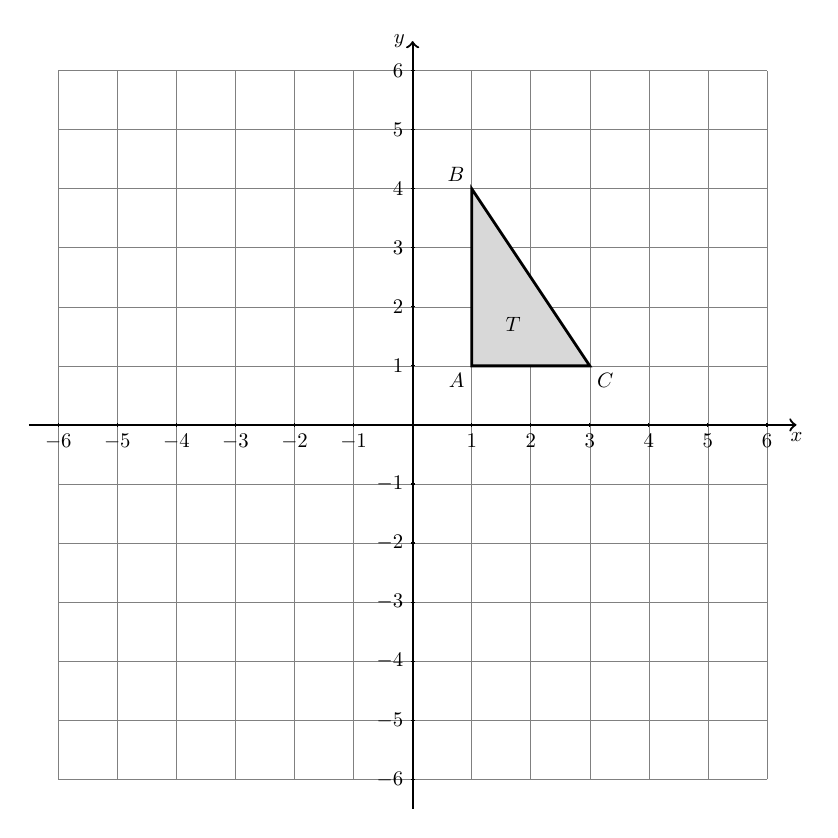
\begin{tikzpicture}[scale=0.75, transform shape]
    \def\axisLimit{6}

    \definecolor{borderColour}{HTML}{000000}
    \definecolor{fillColourT}{HTML}{D8D8D8}

    % Draw grid
    \draw[step=1cm,gray,very thin] (-\axisLimit,-\axisLimit) grid (\axisLimit,\axisLimit);

    % Draw axes
    \draw[thick,->] (-\axisLimit-0.5,0) -- (\axisLimit+0.5,0) node[anchor=north] {$x$};
    \draw[thick,->] (0,-\axisLimit-0.5) -- (0,\axisLimit+0.5) node[anchor=east] {$y$};

    % Label x-axis and y-axis
    \foreach \x in {-\axisLimit,...,-1,1,2,...,\axisLimit}
        \draw (\x cm,1pt) -- (\x cm,-1pt) node[anchor=north] {$\x$};
    \foreach \y in {-\axisLimit,...,-1,1,2,...,\axisLimit}
        \draw (1pt,\y cm) -- (-1pt,\y cm) node[anchor=east] {$\y$};

    % Triangle T: A(1,1), B(1,4), C(3,1)
    \coordinate (A) at (1,1);
    \coordinate (B) at (1,4);
    \coordinate (C) at (3,1);
    \filldraw[fill=fillColourT, draw=borderColour, line width=1pt] (A) -- (B) -- (C) -- cycle;

    \node[below left] at (A) {$A$};
    \node[above left] at (B) {$B$};
    \node[below right] at (C) {$C$};
    \node at (1.7,1.7) {$T$};

\end{tikzpicture}
\end{center}

\noindent On a copy of the grid, rotate triangle $T$ by $90^\circ$ clockwise about the origin $O$.\\
Label the image $T'$, and write down the coordinates of the vertices $A'$, $B'$, $C'$.

\vspace{5cm}

\begin{flushright}
    \answerplain{3}
\end{flushright}
\end{question}
